\section{Description}
IzPack est un générateur d'installeur d'application open-source crée en 2001 par Julien Ponge.
\subsection{Générateur d'installeur}
A partir d'une application cree, Izpack est capable de generer un installateur. Cet installateur pourra etre utilise pour deployer l'application sur n'importe quelle machine. L'interet d'Izpack reside dans le fait que cree une installation est souvent laborieux et n'apporte que peu de plus-value au programme. Izpack propose une solution pour creer cet installeur de maniere simple et universelle. 

Izpack 
Tout type de programme peut etre package, que ce soit une application C++, Java...
\subsection{Open-source}
Izpack est sous license Apache2. Cette license permet l'acces au code source et l'utilisation du logicielle. Il est tout a fait possible de l'utiliser pour une application commerciale voire, de modifier les sources pour correspondre a ses besoins. Une importante communaute s'est regroupee autour de ce projet ce qui a permit son evolution jusqu'a maintenant.

\subsection{Fonctionnalités}
Izpack possède plusieurs fonctionnalités, nous allons en voir les principales :
\subsubsection{multi-plateforme}
Izpack crée un installeur Java. Il suffit donc que la machine ait un machine virtuelle pour pouvoir lancer l'installation, indépendamment de la plateforme et du système d'exploitation.
\subsubsection{Personnalisation}
Izpack possède un ensemble de ``panneaux'' (panel en anglais) qui vont constituer l'installateur graphique. L'aspect global et l'aspect des panels est personnalisable par l'utilisateur via le descripteur XML.
\subsubsection{Internationalisation}
Izpack supporte la création d'installeur multilangues. Pour la localisation, tout repose sur des fichiers XML.
\subsubsection{Installation automatique}
A la fin de l'installation, il est possible de générer un script d'installation automatique. Ce script permet de reproduire l'installation réalisée sur d'autres machines.
\subsection{Popularité}
Izpack est utilisé dans de grand projets comme Jboss, Xwiki, Glassfish... A l'heure actuelle, les téléchargements mensuels s'élèvent a 15.000.
% Image des telechargement?
\section{Architecture}
\subsection{Architecture globale}
Globalement, Izpack possède 2 composants, le compilateur qui va gérer la création de l'installeur et l'installeur.
\subsection{Compilateur}
Le compilateur package l'ensemble des fichiers nécessaires dans un seul fichier jar. Selon la description de l'installation, il va incorporer les panels nécessaires au lancement de celle-ci. 
\subsection{Installeur}
La partie installation concerne toute la logique et la présentation du processus d'installation. 
\subsubsection{Exemples de panels}
Il existe de nombreux types de panels : des panel pour accueillir l'utilisateur et lui afficher des informations (HelloPanel et HTMLInfoPanel), d'autres pour demander à l'utilisateur des informations (UserInputPanel), etc.
Il existe aussi des panels plus spécialisés. Ainsi, CompilePanel permet de compiler du code java, et ProcessPanel permet de lancer des programmes après l'installation.

\section{Exemples d'installation}
De nombreux exemples complexes existent, par exemple l'installeur de IzPack, celui de Glassfish, etc. Pour illustrer simplement l'utilisation de IzPack, utilisons plutôt le petit exemple fourni avec le code de l'application.

\subsection{Description du xml}

% un peu porc comme méthode, copier/coller une partie du xml...
% mais je ne vois pas comment présenter ce xml
% et puis ça suffira, au moins pour un premier jet

Ce xml (install.xml) décrit complètement l'installation.
Une balise info permet de définir les informations concernant l'application : 
\begin{lstlisting}
<info>
	<appname>Sample Installation</appname>
	<appversion>1.4 beta 666</appversion>
	...
</info>
\end{lstlisting}
Une autre balise, guipref permet de définir quelques propriétés de la fenêtre de l'installeur :
\begin{lstlisting}
<guiprefs width="640" height="480" resizable="yes"/>
\end{lstlisting}
Les langues sont définies par la balise locale :
\begin{lstlisting}
<locale>
	<langpack iso3="eng"/>
	<langpack iso3="fra"/>
</locale>
\end{lstlisting}
Des fichiers externes nécessaires à l'installation peuvent être définis par la balise resources :

\begin{lstlisting}
<resources>
	<res id="LicencePanel.licence" src="Licence.txt"/>
</resources>
\end{lstlisting}
Les panels visibles par l'utilisateur sont décrits dans la balise panels :
\begin{lstlisting}
<panels>
	<panel classname="HelloPanel"/>
	...
	<panel classname="FinishPanel"/>
</panels>
\end{lstlisting}
Enfin 
\begin{lstlisting}
<packs>
<pack name="Base" required="yes">
	<description>The base files</description>
	<file src="Readme.txt" targetdir="$INSTALL_PATH"/>
	...
</pack>
<pack name="Docs" required="no">
	...
</pack>
...
</packs>
\end{lstlisting}
Bien sûr d'autres options existent, mais celles présentées ici suffisent à créer notre installeur.
\subsection{Génération du jar}
Pour générer notre installeur, il suffit d'avoir de lancer la commande suivante :
\begin{verbatim}
	compile install.xml
\end{verbatim}
Cette exécution va produire un fichier install.jar : notre installeur.
\subsection{Installation}
Il suffit désormais de lancer le jar pour installer notre application.
\begin{figure}[H]
	\centering
	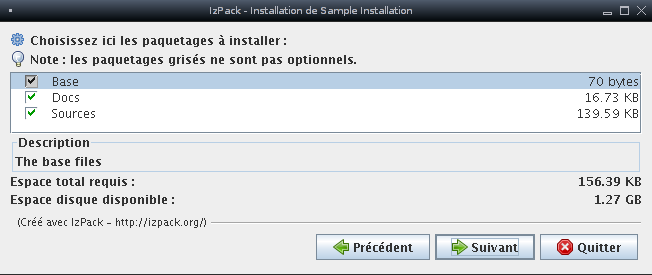
\includegraphics[width=15cm]{../image/installSample.png}
	% installSample.png: 652x275 pixel, 72dpi, 23.00x9.70 cm, bb=0 0 652 275
	\caption{Exemple d'installation avec IzPack}
\end{figure}

\section{Problèmes actuels}
IzPack possède, comme tout logiciel, des bugs potentiels ou des améliorations à effectuer.
Heureusement, sa licence open-source permet à tout développeur d'apporter ses contributions.

\subsection{Nanoxml}
Une amélioration possible concerne la gestion des fichiers XML, qui ont une grande importance dans IzPack.
Pour lire/écrire des fichiers XML, IzPack se base sur une librairie, nanoXML. Cette librairie n'est malheureusement plus mise à jour (la dernière mise à jour date de 2003) et possède encore quelques bugs.
De plus, les versions récentes de l'environnement java (JRE) possèdent de base tout ce qu'il faut pour gérer le xml.
Se débarasser de la dépendance à nanoXML et se reposer uniquement sur la JRE permet donc non seulement de rendre la gestion des XML plus sûre et robuste, mais également de diminuer la taille de l'installeur généré.